\documentclass[a4paper,11pt]{article}

\usepackage[T1]{fontenc}
\usepackage[utf8]{inputenc}
\usepackage{graphicx}
\usepackage{xcolor}

\renewcommand\familydefault{\sfdefault}
\usepackage[defaultmono]{droidmono}

\usepackage{enumerate}
\usepackage{hyperref} 

\usepackage{listings}

\usepackage{geometry}
\geometry{total={210mm,297mm},
left=25mm,right=25mm,%
bindingoffset=0mm, top=20mm,bottom=20mm}


\linespread{1.3}

\newcommand{\linia}{\rule{\linewidth}{0.5pt}}
\renewcommand{\arraystretch}{1.5}
\makeatletter
\renewcommand{\maketitle}{
\begin{center}
\vspace{2ex}
{\huge \textsc{\@title}}
\vspace{1ex}
\\
\linia\\
\@author \hfill \@date
\vspace{4ex}
\end{center}
}
\makeatother

\usepackage{fancyhdr}
\pagestyle{fancy}
\lhead{}
\chead{}
\rhead{}
\lfoot{ChallP FS16}
\cfoot{}
\rfoot{Page \thepage}
\renewcommand{\headrulewidth}{0pt}
\renewcommand{\footrulewidth}{0pt}
%

\begin{document}

\title{GPIO Factsheet}

\author{fbinna, vmeier, laquino}

\date{2016}

\maketitle
\part{Beschreibung GPIO}
\section*{Facts}
\begin{tabular}{| p{3.5cm} | p{10cm} |}
	\hline
	\textbf{Abkürzung} & General Purpose Input/Output\\\hline
	\textbf{Übertragungsraten} & $Taktfrequenz \times Anzahl PINs \times Encoding Bitrate$ \\\hline
	\textbf{Anschluss} & -\\\hline
	\textbf{Topologie} & -\\\hline
	\textbf{Synchron/Asynchron} & Beides möglich\\\hline
	\textbf{Fehlervermeidung} & 5V tolerante Inputs (Prävention gegenüber zu hoher Spannung)\\\hline
	\textbf{Adressierung} & PIN-weise (PINS sind nummeriert)\\\hline
	\textbf{Weitere Geräte} & 
	\begin{itemize}
		\item LEDs
		\item Buzzer
	\end{itemize}
	\\\hline
\end{tabular}
\section*{Generelle Beschreibung}
GPIO steht für "General Purpose Input/Output" und es handelt sich dabei um einen Pin auf einem Integrierten Schaltkreis, welcher keiner bestimmten Funktion zugeordnet ist, sondern vom Benutzer des Geräts nach Wünschen eingesetzt werden kann. Als GPIO Port wird eine Menge von typischerweise 8 Pins bezeichnet, welche als Gruppe kontrolliert werden. Ports oder einzelne PINs können als Input oder Output konfiguriert werden und disabled beziehungsweise enabled werden. \\
Ein Pin kann die Werte 1 (High) oder 0 (Low) entsprechend der Spannung annehmen. Eine Port von 8 Pins kann also Werte von 0 (00000000) bis 255 (11111111) parallel übertragen.
	
\section*{GPIO auf dem Raspberry Pi}
\subsection*{Betriebsspannung}
GPIO funktioniert für verschiedene Spannungslevels (meist zwischen 2V und 5V). Das Raspberry arbeitet mit max. 3.3V Spannung für diese PINS. Während eine Schreiboperation auf 5V-GPIO-Geräte möglich ist, muss beachtet werden, dass dieses Gerät seinerseits keine Schreiboperation auf die PINS des Raspberrys ausführt.

\subsection*{PIN Nummerierung}
Das Raspberry unterstützt grundlegend zwei Modi, über welche die GPIO PINS angesteuert werden.
\begin{tabular}{| p{2cm} | p{7cm} | p{7cm} | }
	\hline
	\textbf{} & \textbf{Vorteile} & \textbf{Nachteile} \\\hline
	\textbf{BCM} & 
			\begin{itemize}
				\item Universelle Nummerierung (Broadcomm SoC numbering)
				\item Unabhängig von Programmiersprache
			\end{itemize}~& 
			\begin{itemize}
				\item Unintuitiv (keine ersichtliche Reihenfolge o.ä.)
				\item Nummerierung von Gerät abhängig (Raspberry Pi 1 ist anders als Raspberry Pi 2)
			\end{itemize}~\\
	&
	\multicolumn{2}{|c|}{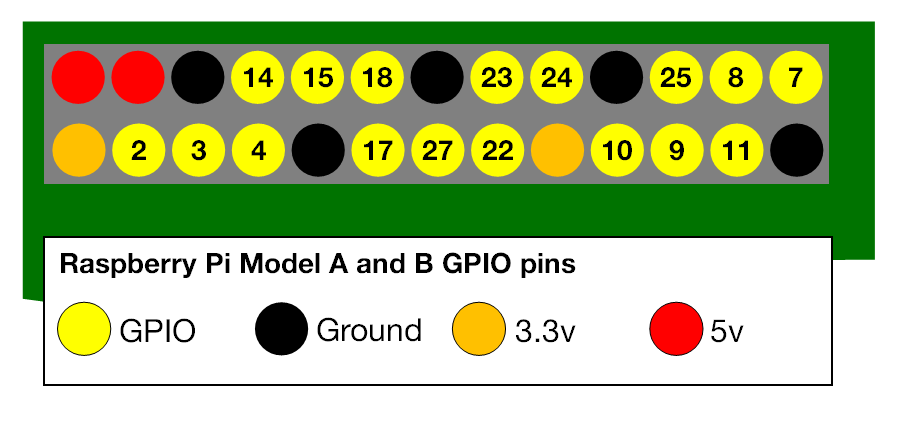
\includegraphics[width=0.49\textwidth]{images/bcm.png}}~\\\hline
	
	\textbf{BOARD} & 
		\begin{itemize}
			\item Einfache Durchnummerierung der PINS
			\item Gerätunabhängige Nummerierung
		\end{itemize}~& 
		\begin{itemize}
			\item PIN 5 auf Raspberry Pi 1 hat möglicherweise andere Funktion als PIN 5 auf Raspberry Pi 2
		\end{itemize}~
	\\
	&
	\multicolumn{2}{|c|}{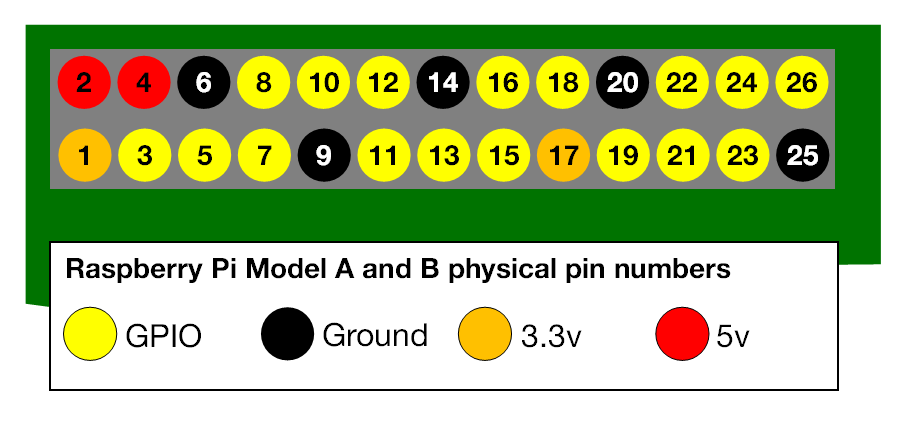
\includegraphics[width=0.49\textwidth]{images/board.png}}~\\\hline
	
\end{tabular}

\subsection*{Übertragungs-Modi}
Für eine Übertragung von Daten oder Zeichen an ein Interface sind zwei Modi verfügbar, der 4Bit- und der 8Bit-Modus. Über einen GPIO PIN wird jeweils ein Bit übertragen, was bedeutet, dass im 4Bit-Modus 4 Verbindungen und im 8Bit-Modus 8 Verbindungen nötig sind.\par
Während im 8Bit-Modus alle Zeichen gleichzeitig übertragen werden können, muss der 4Bit Modus ein Byte aufsplitten, indem zuerst die höheren 4Bit und darauffolgend die tieferen 4Bit übertragen werden.

\part{Beschreibung LCD Display (HD44780 kompatibel)}
\section*{Facts}
\begin{tabular}{| p{3.5cm} | p{10cm} |}
	\hline
	\textbf{Dateninput-Modus} & 4Bit / 8Bit Modus\\\hline
	\textbf{Eingangsspannung} & 
	\begin{itemize}
		\item $V_{dd}$ (Logik-Energiesupply): -0.3V bis 6V
		\item $V_{lcd}$ (LCD-Energiesupply): $V_{dd}-11.5V$ bis $V_{dd}+0.3V$
		\item $V_{i}$ (Eingangsspannung): -0.3V bis $V_{dd} + 0.3V$
	\end{itemize}~
	\\\hline
	\textbf{Taktrate} & Entspricht Konfiguration der MPU; 2MHz bei 5V Eingangsspannung\\\hline
	\textbf{LCD Matrix} & $5 \times 8$ Matrix\\\hline
	\textbf{Display RAM} & $80 \times 8$-bit (max. 80 Characters)\\\hline
	\textbf{Treiber} & Betrieb mit HD44780-Treiber möglich\\\hline
\end{tabular}

\section*{Instruktionsset Beispiel}
\subsection*{8Bit Modus}
\begin{tabular}{| c | c | l |}
	\hline
	\textbf{RS} & \textbf{D7 bis D0} & \textbf{Beschreibung} \\\hline
	0 & 0 0 1 1 - 1 0 0 0 & 8Bit-Modus, 2 Linien, $5 \times 7$ Matrix \\\hline
	0 & 0 0 0 0 - 1 1 1 1 & Display ON, Cursor ON, Blinkender Cursor \\\hline
	0 & 0 0 0 0 - 0 1 1 0 & Entry Mode, Cursor Position heraufzählen, Kein Display Shift\\\hline
	1 & \ldots & 8Bit Repräsentation Character\\\hline
\end{tabular}

\subsection*{4Bit-Modus}
Im 4Bit-Modus sind die PINs D3 bis D0 geerdet, Instruktionen erfolgen nur über PINs D7 bis D4.
\begin{tabular}{| c | c | l |}
	\hline
	\textbf{RS} & \textbf{D7 bis D0} & \textbf{Beschreibung} \\\hline
	0 & 0 0 1 0 - 0 0 0 0 & 4Bit-Modus (1 nibble Operation)\\\hline
	0 & 0 0 1 0 - 0 0 0 0 & 8Bit-Instruktionsset \\\hline
	0 & 1 0 0 0 - 0 0 0 0 & Zweiter Nibble \\\hline
	
	0 & 0 0 0 0 - 0 0 0 0 & Display ON, Cursor ON, Blinkender Cursor\\\hline
	0 & 1 1 1 1 - 0 0 0 0 & Zweiter Nibble \\\hline
	
	0 & 0 0 0 0 - 0 0 0 0 &  Entry Mode, Cursor Position heraufzählen, Kein Display Shift\\\hline
	0 & 0 1 1 0 - 0 0 0 0 & Zweiter Nibble \\\hline
		
	
	
	1 & \ldots & Erste 4Bit der 8Bit Character Repräsentation \\\hline
	1 & \ldots & Zweite 4Bit der 8Bit Character Repräsentation \\\hline
\end{tabular}

\newpage

\section*{Codebeispiel}
Dieses Codebeispiel zeigt auf einfache Art wie GPIO grundsätzlich funktioniert. Am Pin 18 ist eine LED und an Pin 11 ein Button angeschlossen.
Die While-Schlaufe setzt den Pin 18 auf 255 (true) falls der Button gedrückt wird und umgekehrt.\\

\lstinputlisting[language=Python, frame=single]{GPIO-Example.py}
Mit GPIO.setup kann ein Pin als Input oder Ouput definiert werden. Mit GPIO.input oder GPIO.output kann der Wert eines Pins gelesen bzw. gesetzt werden.


\section*{Quellen}
\href{https://en.wikipedia.org/wiki/General-purpose_input/output}{Wikipedia Artikel zu GPIO}\\
\href{http://www.mikrocontroller.net/articles/HD44780}{Mikrocontroller.net Beschreibung zu HD44780}\\
\href{http://makezine.com/projects/tutorial-raspberry-pi-gpio-pins-and-python/}{Makezine GPIO Tutorial (u.a. über PIN Modi)}\\
\href{https://projects.drogon.net/raspberry-pi/gpio-examples/lcd-interface/}{Artikel zu LCD Displays am Raspberry Pi}\\
\href{https://www.sparkfun.com/datasheets/LCD/HD44780.pdf}{Datasheet HHD44780}\\
\href{http://www.protostack.com/download/YJD1602A-1\%20datasheet.pdf}{Datasheet Arduino LCD Modul}\\
\href{http://www.protostack.com/blog/2010/03/character-lcd-displays-part-1/}{LCD Ansteuerung 8Bit- und 4Bit-Modus}\\
\href{http://openmicros.org/index.php/articles/94-ciseco-product-documentation/raspberry-pi/217-getting-started-with-raspberry-pi-gpio-and-python}{Raspberry Pi und GPIO Tutorial}

\end{document}
